


\chapter{Numerical Results}
  \label{ch_results}

\todo{This chapter is the real moneymaker. The overarching motivation for this work is that Pc4 pulsations vary in interesting ways with respect to azimuthal modenumber, and that prior models have been unable to give a good picture of that behavior. }

%\todo{Do we every check E/B against $\Sigma_P / \mz$? }

%\todo{Do we see a difference between \vec{k} (momentum) and the group velocity? Poynting flux will always be pretty much along the field line, since $B_3$ is small and $E_3$ is zero, but the wave vector need not be. This is a question of coupling/converting to compressional waves, I guess. }

%\todo{Look at McKenzie and Westphal. Waves incident on the bow shock, etc, at weird angles. }

%\todo{Look at the E to B ratio. Compare to the \Alfven speed and to the height-integrated Pedersen conductivity. }

% -----------------------------------------------------------------------------
% -----------------------------------------------------------------------------
% -----------------------------------------------------------------------------
\section{Finite Poloidal Lifetimes}
  \label{sec_lifetimes}

In his 1974 paper, Radoski argues that a poloidally-polarized wave should asymptotically rotate to the toroidal polarization\cite{radoski_1974} as a result of the curved derivative in the meridional plane. The question of finite poloidal lifetimes is considered further in a 1995 paper by Mann and Wright\cite{mann_1995}. Their numerical work used a straightened field line, with an \Alfven speed gradient in the ``radial'' direction. They also found a rotation over time from poloidal to toroidal polarization, with the characteristic time proportional to the azimuthal modenumber. 

\todo{Ding et al\cite{ding_1995} did similar work just before Mann and Wright, but results were less clear, possibly due to issues with grid resolution (as discussed in \cite{mann_1995}). }

\todo{Mann and Wright looked specifically at second harmonics. This work is on first harmonics. (In principle Tuna allows arbitrary driving waveforms and spatial distributions.) }

The present section builds on the aforementioned results by relaxing several of their nonphysical assumptions. First, Tuna's geometry (as described in \cref{ch_model}) is far more realistic than Radoski's half-cylinder or the box model used by Mann and Wright. Magnetic field lines are dipolar. \Alfven speed is based on an empirical profile, and varies along and across field lines. Next, the present results feature driving delivered over time through perturbation of the ring current; past work has instead considered the evolution of an initial condition. Finally, the present model includes a height-resolved ionosphere (rather than perfectly-reflecting boundaries). The ionospheric conductivity provides a direct coupling between the poloidal and toroidal modes, in addition to dissipating energy. 

Each subplot in \cref{fig_U_day,fig_U_day_nosigh,fig_U_day_big,fig_U_night} is analogous to Mann's Figure 3. Blue lines show the total energy in the poloidal mode as a function of time. Red lines show toroidal energy. Runs are organized such that driving frequency is constant down each column, and azimuthal modenumer is constant across each row. Axis bounds are held constant across all subplots. 

Energy is computed per Poynting's theorem, with due consideration of the unusual geometry. Energy density is integrated over the meridional plane, but not in the azimuthal direction, giving units of gigajoules per radian; more than anything else, this serves as a reminder that the waves under consideration are azimuthally localized. 
\begin{align}
  \label{def_energy}
  U_P &= \displaystyle\int \frac{d\lysakx d\lysakz}{2 \mz \jac} \lr{ B_x^2 + \frac{1}{\va^2} E_y^2} &
  U_T &= \displaystyle\int \frac{d\lysakx d\lysakz}{2 \mz \jac} \lr{ B_y^2 + \frac{1}{\va^2} E_x^2} 
\end{align}

The twenty-eight runs shown in \cref{fig_U_day} use a high-conductivity profile, corresponding to the dayside with high solar activity. 

\begin{figure}[!htb]
    \centering
    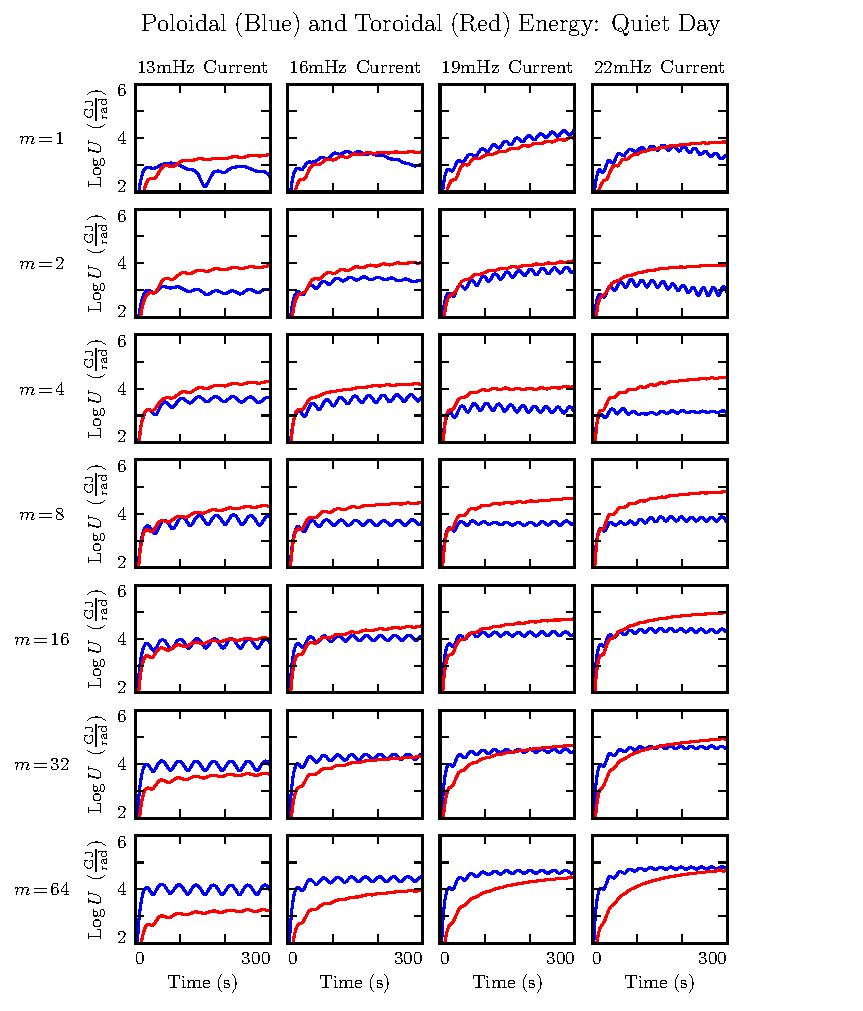
\includegraphics[width=\textwidth]{figures/U_day.pdf}
    \caption[Poloidal and Toroidal Energy: Quiet Day]{
      \todo{MAKE THIS PLOT WITH MODEL 2. }
    }
    \label{fig_U_day}
\end{figure}

The fact that \cref{fig_U_day} includes red (toroidal energy) curves at all speaks to the coupling of the poloidal and toroidal modes. As discussed in \cref{ch_model}, driving in Tuna is delivered purely into the poloidal electric field (as a proxy for the azimuthal current). 

As expected, the rotation from poloidal to toroidal is slowest at large azimuthal modenumbers. The toroidal energy overtakes the poloidal energy within a single drive period at $\azm=4$; with $\azm=64$, the most of the energy is in the poloidal mode for \about10 driving periods. However, the relationship between azimuthal modenumber and rotation timescale is not linear, as was suggested by Mann and Wright. Instead, the rotation is fastest at $\azm=4$. 

This hints at two competing effects. \todo{NOT the Hall conductivity. The same effect is present when the runs are repeated with $\sh=0$. It's actually energy escaping to the outer boundary! $\azm\sim4$ is where the \Alfven wave stops being compressional near where the driving is delivered. Note that higher frequency driving should be MORE prone to losing energy to the sides. Not clear that's the case. }

\todo{While the Hall conductivity does in principle allow energy to move from the toroidal mode back to the poloidal mode, the rate does not seem to be significant. In the rightmost column of \cref{fig_U_day}, the toroidal mode holds more energy than the poloidal mode by two orders of magnitude, yet there is no indication of the poloidal mode picking up energy to catch up. }

The total energy in the system is asymptotically determined by the balance between the energy input (from driving) and the energy loss (through Joule dissipation in the ionosphere). When the driving frequency is not particularly close to the local \Alfven frequency, the energy reaches its asymptotic value quickly. When those frequencies align closely, energy accumulates over a larger number of drive periods, and the asymptotic value is larger. 

The system's resonant frequency (for a fundamental poloidal mode at $L=5$) is affected significantly by the size of the plasmasphere. In \cref{fig_U_day}, with the plasmapause at $L_{PP}=4$, the system resonates at \SI{19}{\mHz} at low \azm; as \azm becomes large, the resonant frequency is closer to \SI{22}{\mHz}. \cref{fig_U_day_big} shows the effect of moving the plasmapause to $L_{PP}=5$: resonance is closer to \SI{16}{\mHz}. The runs are otherwise identical to those shown in \cref{fig_U_day}. 

\begin{figure}[!htb]
    \centering
    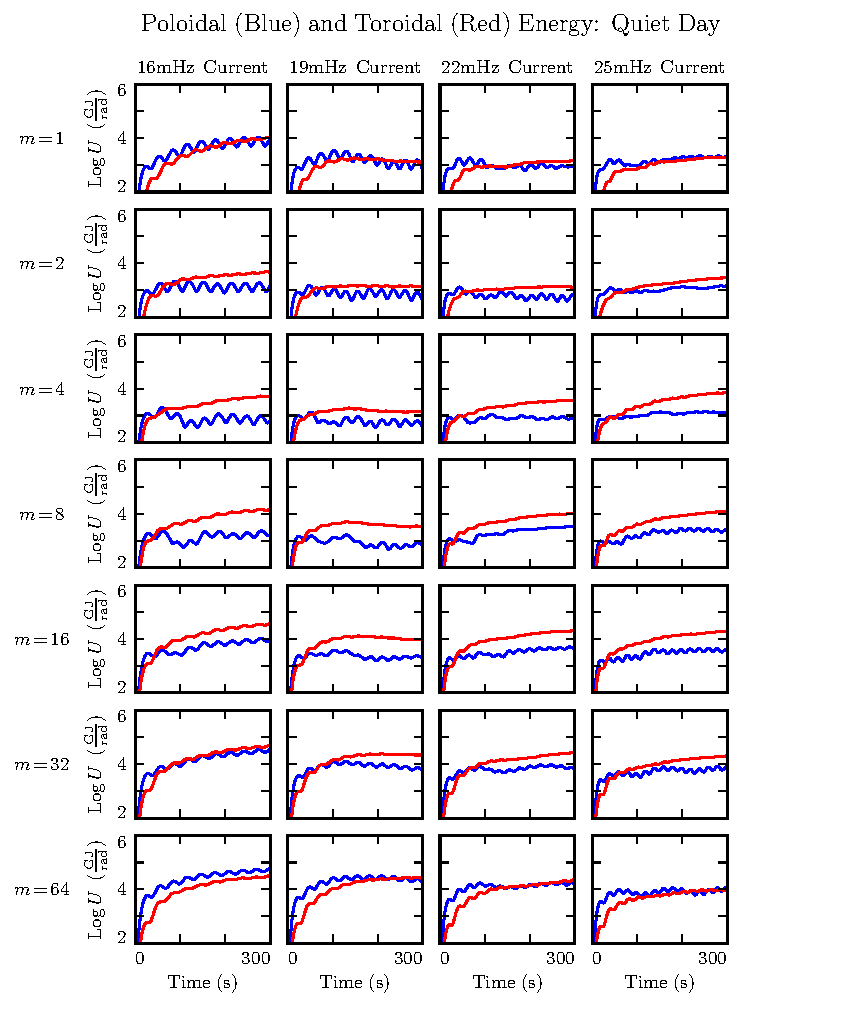
\includegraphics[width=\textwidth]{figures/U_day_big.pdf}
    \caption[Poloidal and Toroidal Energy: Quiet Day, Large Plasmasphere]{
      Changing the position of the plasmapause has a significant effect on the \Alfven bounce time. \todo{FIX PLOT TITLE. } 
    }
    \label{fig_U_day_big}
\end{figure}

On the nightside, the picture changes significantly. 

The ionospheric conductivity on the nightside is lower. As a result, energy is dissipated more efficiently. 

\todo{The asymptotic energy -- at which driving and dissipation balance -- is much lower on the nightside. It's reached much more quickly as a result. The system does not accumulate energy over multiple driving periods. }

\todo{The system resembles a damped-driven oscillator. There is no evidence of resonance -- of an energy buildup over multiple driving periods. Instead, the energy follows the waveform of the driver. }

\todo{The only difference between the runs shown in \cref{fig_U_day} and those in \cref{fig_U_night} is the ionospheric profile. }

\todo{Rotation of poloidal energy to the toroidal mode is present on the nightside, as it is on the dayside. There's less energy, of course, because the ionosphere damps the poloidal mode just as fast as it can rotate. The toroidal mode also doesn't last long, since the ionosphere damps it as fast as it grows. }

\todo{The rotation rate is shown by the asymptotic division of energy between the poloidal and toroidal modes. As on the dayside, the toroidal mode grows most quickly at $\azm=4$; the poloidal and toroidal modes hold a similar amount of energy. At $\azm=64$, the dissipation timescale is evidently much faster than the rotation timescale... only \about\SI{1}{\percent} of the poloidal energy ever rotates to the toroidal mode. }

\begin{figure}[!htb]
    \centering
    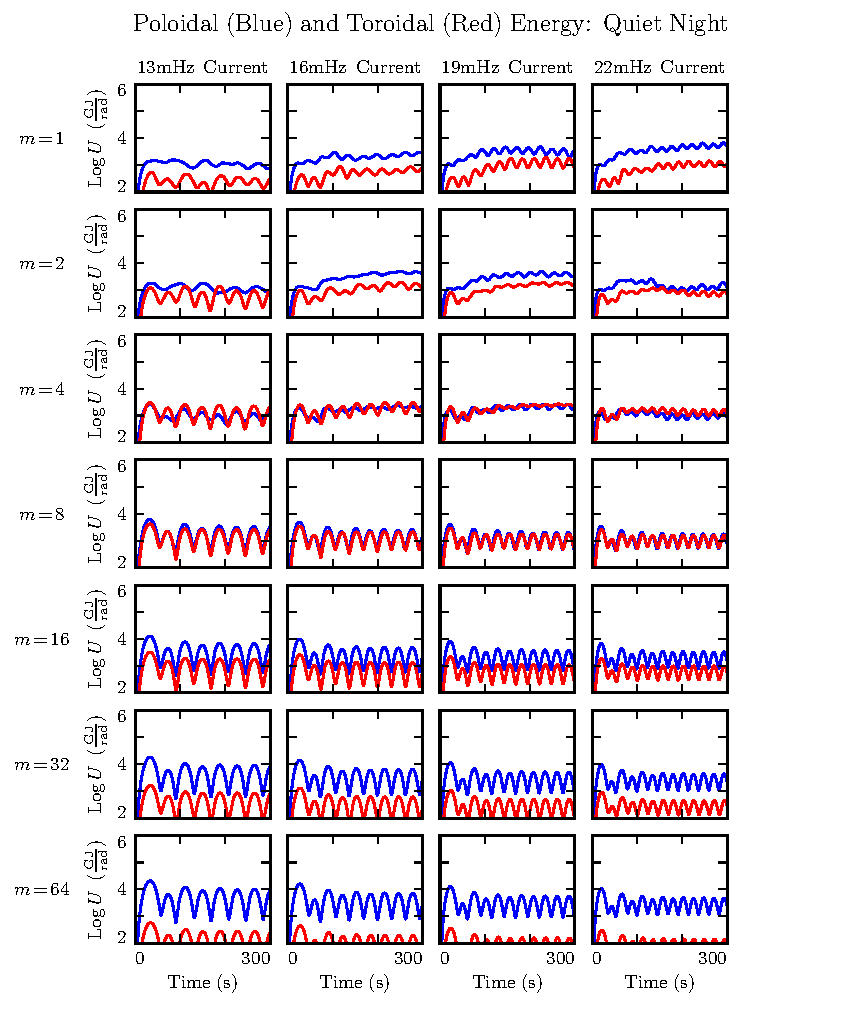
\includegraphics[width=\textwidth]{figures/U_night.pdf}
    \caption[Poloidal and Toroidal Energy: Quiet Night]{
      \todo{REDO WITH MODEL 2. }
%      Driving is applied to the poloidal electric field. There is some rotation of energy to the toroidal mode (and less at high azimuthal modenumber), but the low ionospheric conductivity prevents energy from accumulating over time. 
    }
    \label{fig_U_night}
\end{figure}

The results of the present section show agreement with -- and significant refinement of -- earlier work. In the case of large-but-finite ionospheric conductivity, dipole geometry, and realistic \Alfven speed profile, energy rotates asymptotically from the poloidal mode to the toroidal mode. The rotation rate is strongly affected by azimuthal modenumber and, in the case of large-but-finite \azm, has a characteristic timescale in the tens of periods. 

The present work furthermore considers the issue of poloidal lifetimes in the low conductivity regime (while past work has used perfectly-reflecting boundaries). The result is novel: rather than asymptotically accumulating energy in the toroidal mode, an FLR on the nightside does not seem to accumulate energy at all. This is relevant to the question of day-night asymmetry in the observation of field line resonances. 

% -----------------------------------------------------------------------------
% -----------------------------------------------------------------------------
% -----------------------------------------------------------------------------
\section{Spatial Distribution of Energy}
  \label{sec_layers}

Looking a bit deeper, it's possible to comment on the structure of the poloidal and toroidal modes, not just their magnitudes. 

\todo{Probably should at least mention the nightside? It seems silly to leave it out. }

In the following figures, energy density is computed at each grid point, then averaged over the volume of the flux tube (again, with proper respect to the unusual geometry). This allows the eyeballing of how energy moves across field lines as a function of time. The color scale is shared across all plots. 

Poloidal and toroidal energy are again considered separately. The two exhibit qualitatively different behavior. 

\todo{At low \azm, energy rotates out of the poloidal mode so quickly that no resonance can form. }

\todo{At high \azm, the \Alfven wave is guided. If the driving frequency lines up with the resonant frequency where it's delivered, the poloidal mode resonates strongly. Otherwise, again, no energy accumulates. }

\todo{In no case does the poloidal mode demonstrate the ability to move energy across magnetic field lines. }

\todo{On the other hand, the toroidal mode does resonate, even if the driving isn't resonant (though in that case the response is of course stronger). The toroidal mode transports energy across field lines until it encounters resonance, then accumulates energy there. Often, resonances are seen in multiple locations due to the non-monotonic \Alfven bounce frequency as a function of $L$. }

% RESONANT DRIVING

\begin{figure}[!htb]
    \centering
    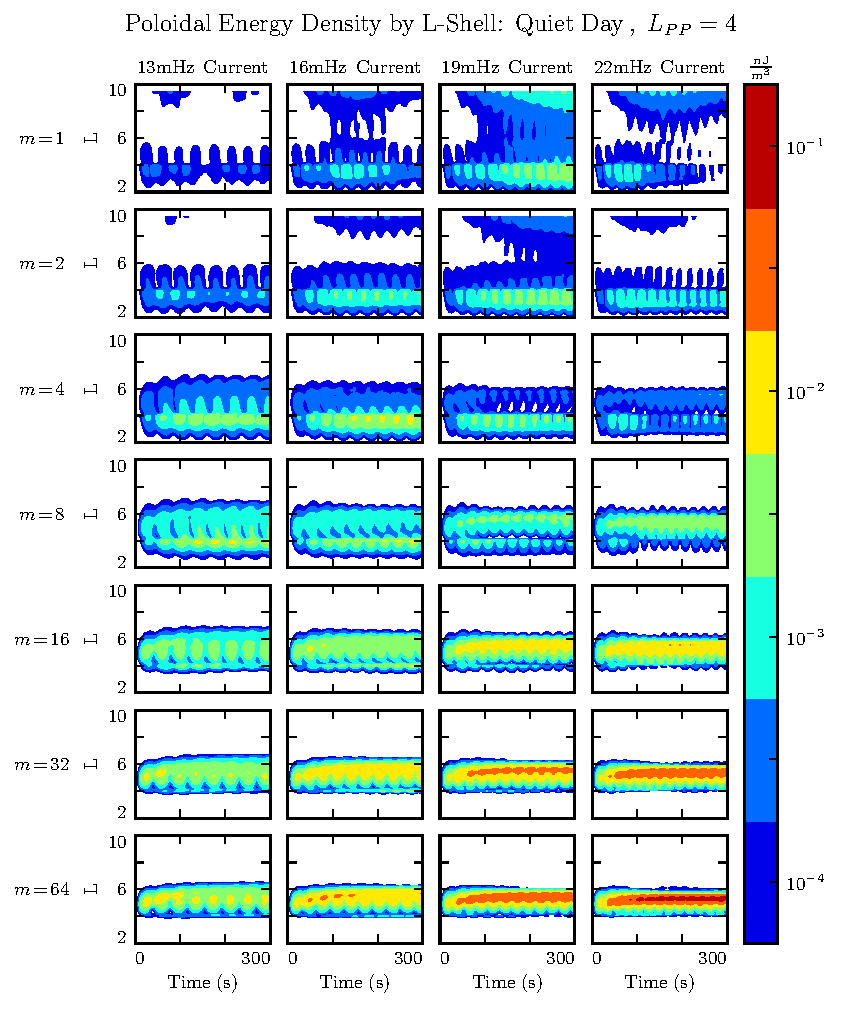
\includegraphics[width=\textwidth]{figures/layers_p_2.pdf}
    \caption[Radial Distribution of Poloidal Energy]{
      \todo{$\cdots$}
    }
    \label{fig_p_layers}
\end{figure}

\todo{If \azm is small, energy rotates to the toroidal mode too fast to form a poloidal resonance. If \azm is large, the \Alfven wave is guided, so it resonates only if the driving frequency lines up with the resonant frequency where it's applied. The result is just one big -- or perhaps even giant -- pulsation. If the driving lines up with a nearby field line, the toroidal mode goes crazy! Resonance inside the plasmasphere. Resonance at the plasmapause. Resonance at the driving location. And (weak) attempt at a higher harmonic further out. }

\todo{When the driving frequency doesn't line up with the location where it's delivered, there's basically no response. There is no movement of energy to a resonant field line, so no energy can accumulate over the course of multiple rounds of driving. Even when not driven resonantly, the toroidal mode still makes the best of its situation. It steals what energy it can from the poloidal mode, carries it to the resonant $L$-shell, and gets to work. (In contrast, recall from \cref{fig_resonant_driving}, in this situation the poloidal mode just does not accumulate energy.) }

\todo{Why is this exciting? }

\todo{Driving from inside the magnetosphere is novel. }


\begin{figure}[!htb]
    \centering
    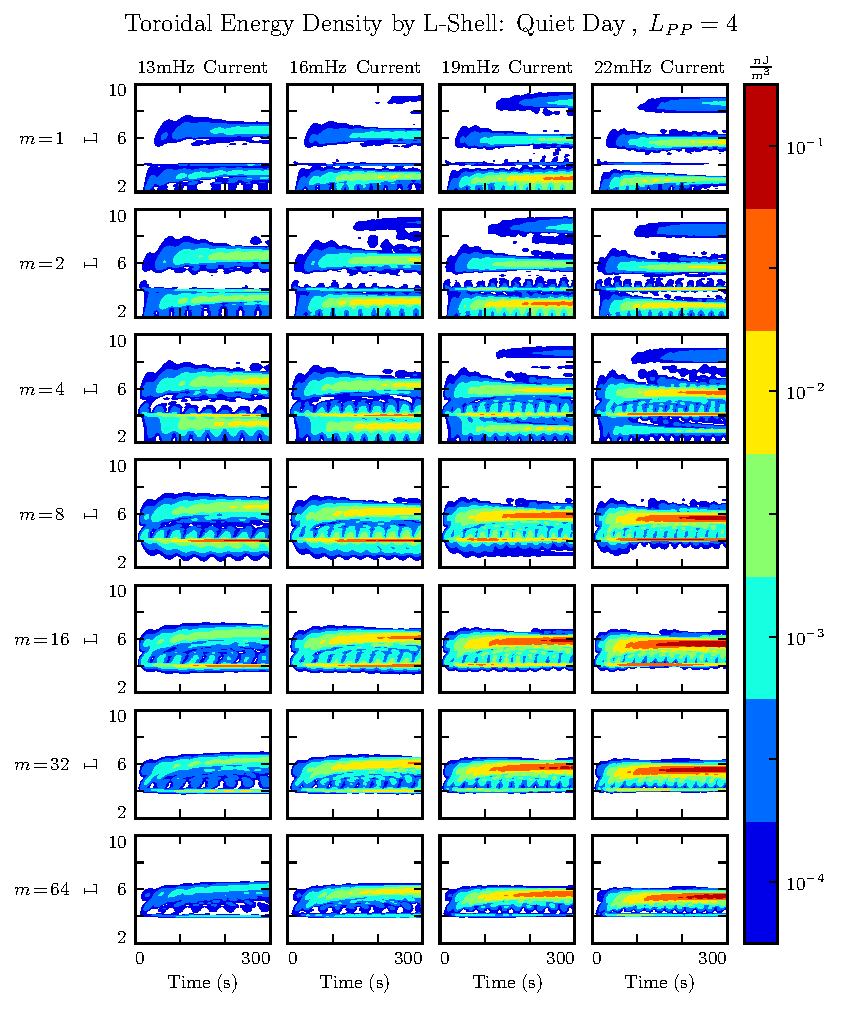
\includegraphics[width=\textwidth]{figures/layers_t_2.pdf}
    \caption[Radial Distribution of Toroidal Energy]{
      \todo{$\cdots$}
    }
    \label{fig_t_layers}
\end{figure}

\todo{Why is this exciting? }









% =============================================================================
% =============================================================================
% =============================================================================
\section{Significance for Giant Pulsations}
  \label{sec_pgs}

Giant pulsations are (probably\cite{takahashi_2011}) fundamental mode poloidal Pc4 pulsations with frequencies around \SI{10}{\mHz} and azimuthal modenumbers around \num{20}. They are large, and can sometimes be observed on the ground. 

While this model makes no particular distinction between a giant pulsation and any other Pc4, the above results do line up with giant pulsation observations. 

Giant pulsations aren't seen at small \azm. As shown in \cref{sec_lifetimes}, low-\azm poloidal modes rotate to the toroidal mode too quickly to resonate effectively, even in the case of continuous driving at a locally-resonant frequency. The sweet spot seems to be around $\azm = 20$, more or less the same point where resonance becomes visible in \cref{fig_resonant_driving}. Admittedly, giant pulsations are typically closer to \SI{10}{\mHz} than \SI{22}{\mHz}. It seems likely that qualitatively similar results would be encountered if the driving were moved to an $L$-shell with a bounce time of \SI{10}{\mHz}. 


\todo{Present profiles do not allow a distinction between the dawn and dusk flank. Future work... Tuna could easily accept new profiles! }


% GROUND SIGNATURES

\todo{\cite{takahashi_2011} talks significantly about the east-west polarization. }

Giant pulsations are seen at very large \azm, though not on the ground\cite{takahashi_2013}, due to damping by the ionosphere. 

Giant pulsations are most common on the dayside (particularly the morningside), during geomagnetically quiet times. Giant pulsation ground signatures are noted for their predisposition towards east-west polarization. 

In \cref{fig_ground_signatures}, the strongest east-west ground signatures is obtained on the geomagnetically quiet dayside, at \azm of 16 and 32. 

This seems to be a giant pulsation ``sweet spot'': the poloidal mode becomes stronger as \azm increases, but the ionospheric damping also increases. 

\begin{figure}[H]
    \centering
    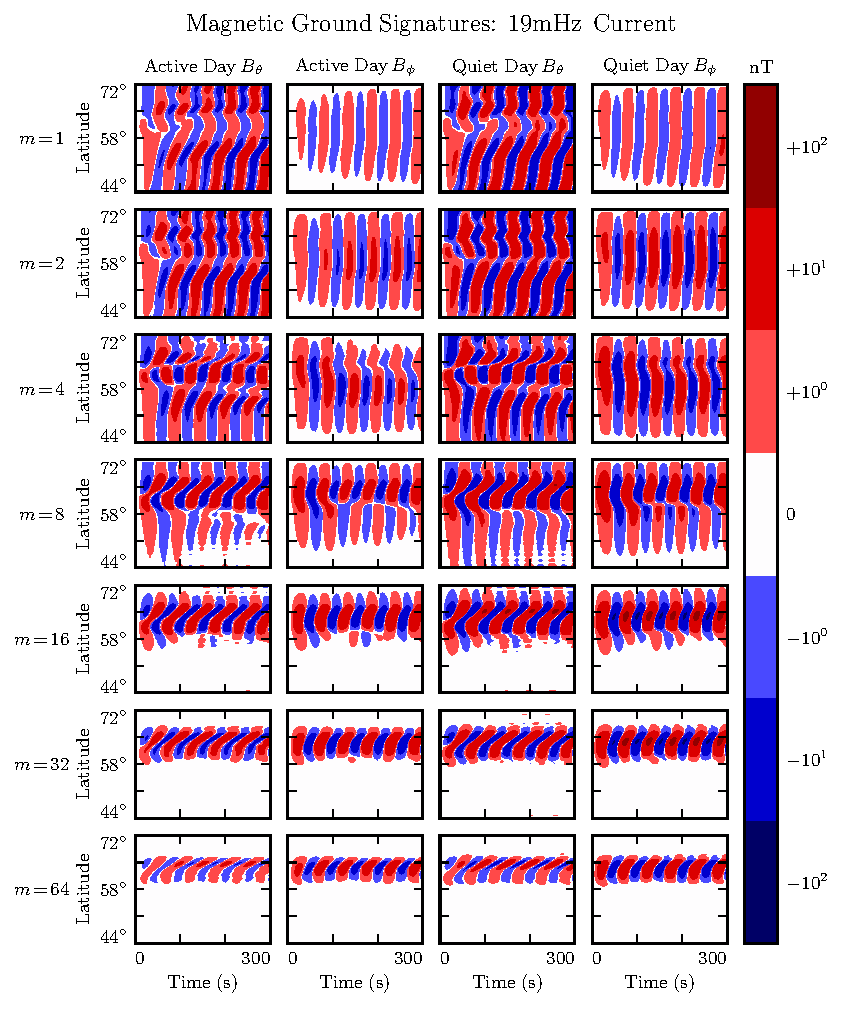
\includegraphics[width=\textwidth]{figures/ground_19mHz.pdf}
    \caption[Dayside Ground Magnetic Fields]{
      The east-west component of magnetic ground signatures is peaked on the geomagnetically quiet dayside, at modenumbers around 16 to 32. This coincides nicely with observations of giant pulsations. Like the east-west component, the north-south ground signature is strongest on the quiet dayside; however, unlike the east-west component, the north-south component is weak when the modenumber is large. 
    }
    \label{fig_ground_signatures}
\end{figure}

Giant pulsations are monochromatic, and can be accompanied by ``multiharmonic toroidal waves''\cite{takahashi_2011}. Per \cref{sec_layers}, this is about what would be expected from a mishmash of poloidal driving. Poloidal modes of all frequencies rotate into the toroidal mode; resonant poloidal modes resonate; non-resonant poloidal modes become evanescent. 

Giant pulsations often drift azimuthally. This model can't resolve azimuthal drift directly, of course, but can fake it by looking at complex phase. There has been some indication (not shown) of complex phase rotation in ground magnetic fields. However, at the boundary, it's difficult to disentangle which values are imaginary to indicate an azimuthal offset, and which are imaginary because of Hall coupling. Investigation is ongoing. 
















